\chapter{Full production process} \label{Full production process}

The industrial practice of producing a fuel tank part through the Extrusion Blow-Molding requires the following stages:

% Provide a two lines description
\begin{itemize}
    \item Material Supply: It constitutes all the equipment needed to provide the Extrusion Blow-Molding machine the raw material/s. 
    \item \textbf{Extrusion Blow-Molding}:
    \item Post Cooling; 
    \item Finishing: 
    \item Assembly:
\end{itemize}



Blow-molding is the first process to produce the fuel system. Once it has been blown, the flash around the tank is removed and regrinded, then it enters a phase of post-mold cooling, where its temperature is lowered with a water flow in a second mold. It is then stabilized in ambient air, before entering the finishing center, where parts of the tank will be cut, and extra components welded on it.
Then some parts will be assembled on the tank, such as the filler pipe presented above. Finally, every tank is tested to detect possible leaks.

The full process is detailed in Figure \ref{fig:Full_production_process}.

\begin{figure}
\centerline{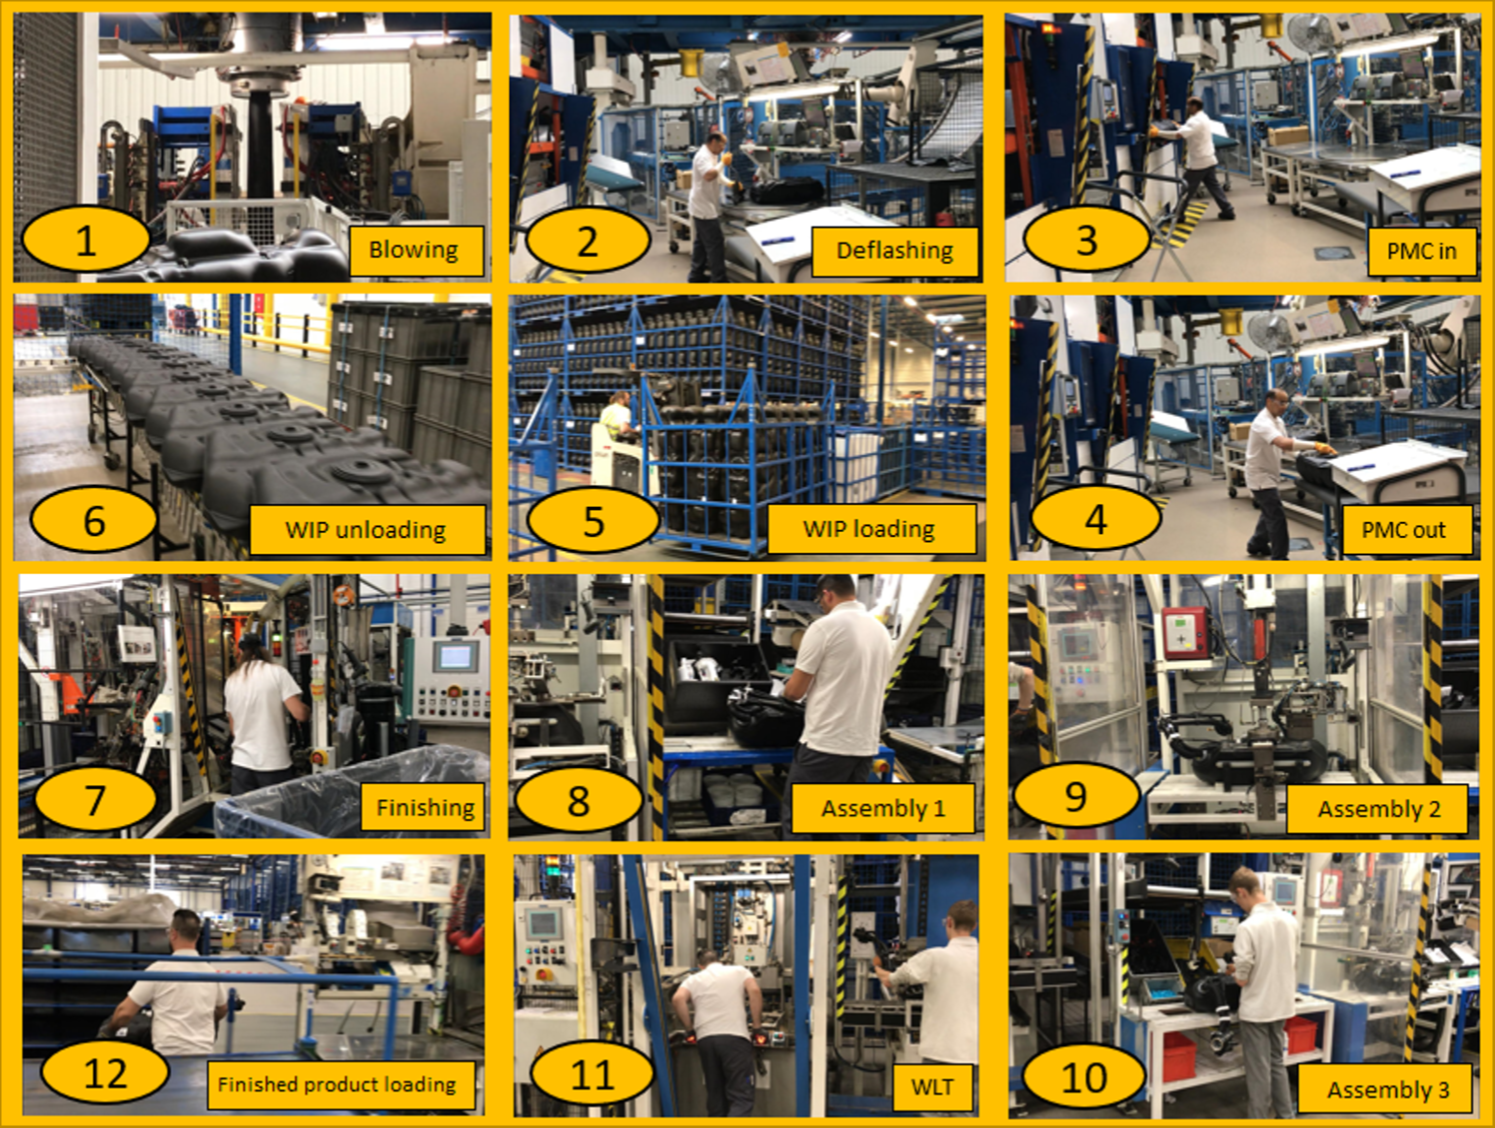
\includegraphics[scale=0.4]{images/appendix_B/Blow_molding_process.png}}
\caption{Full production process}
\label{fig:Full_production_process}
\end{figure}